\chapter{Diagramas de Sequência} \label{cha:diagramassequencia}

%Neste capítulo é apresentado o diagrama de classes.

%DUVIDA: explicação pro diagram?
%DUVIDA: precisa de todos os casos de uso,? sendo que alguns ja tao dentro um do outro

\section{Buscar produto}
\begin{figure}[H]
    \caption{\label{fig:label} DIAGRAMA DE SEQUÊNCIA BUSCAR PRODUTO}
    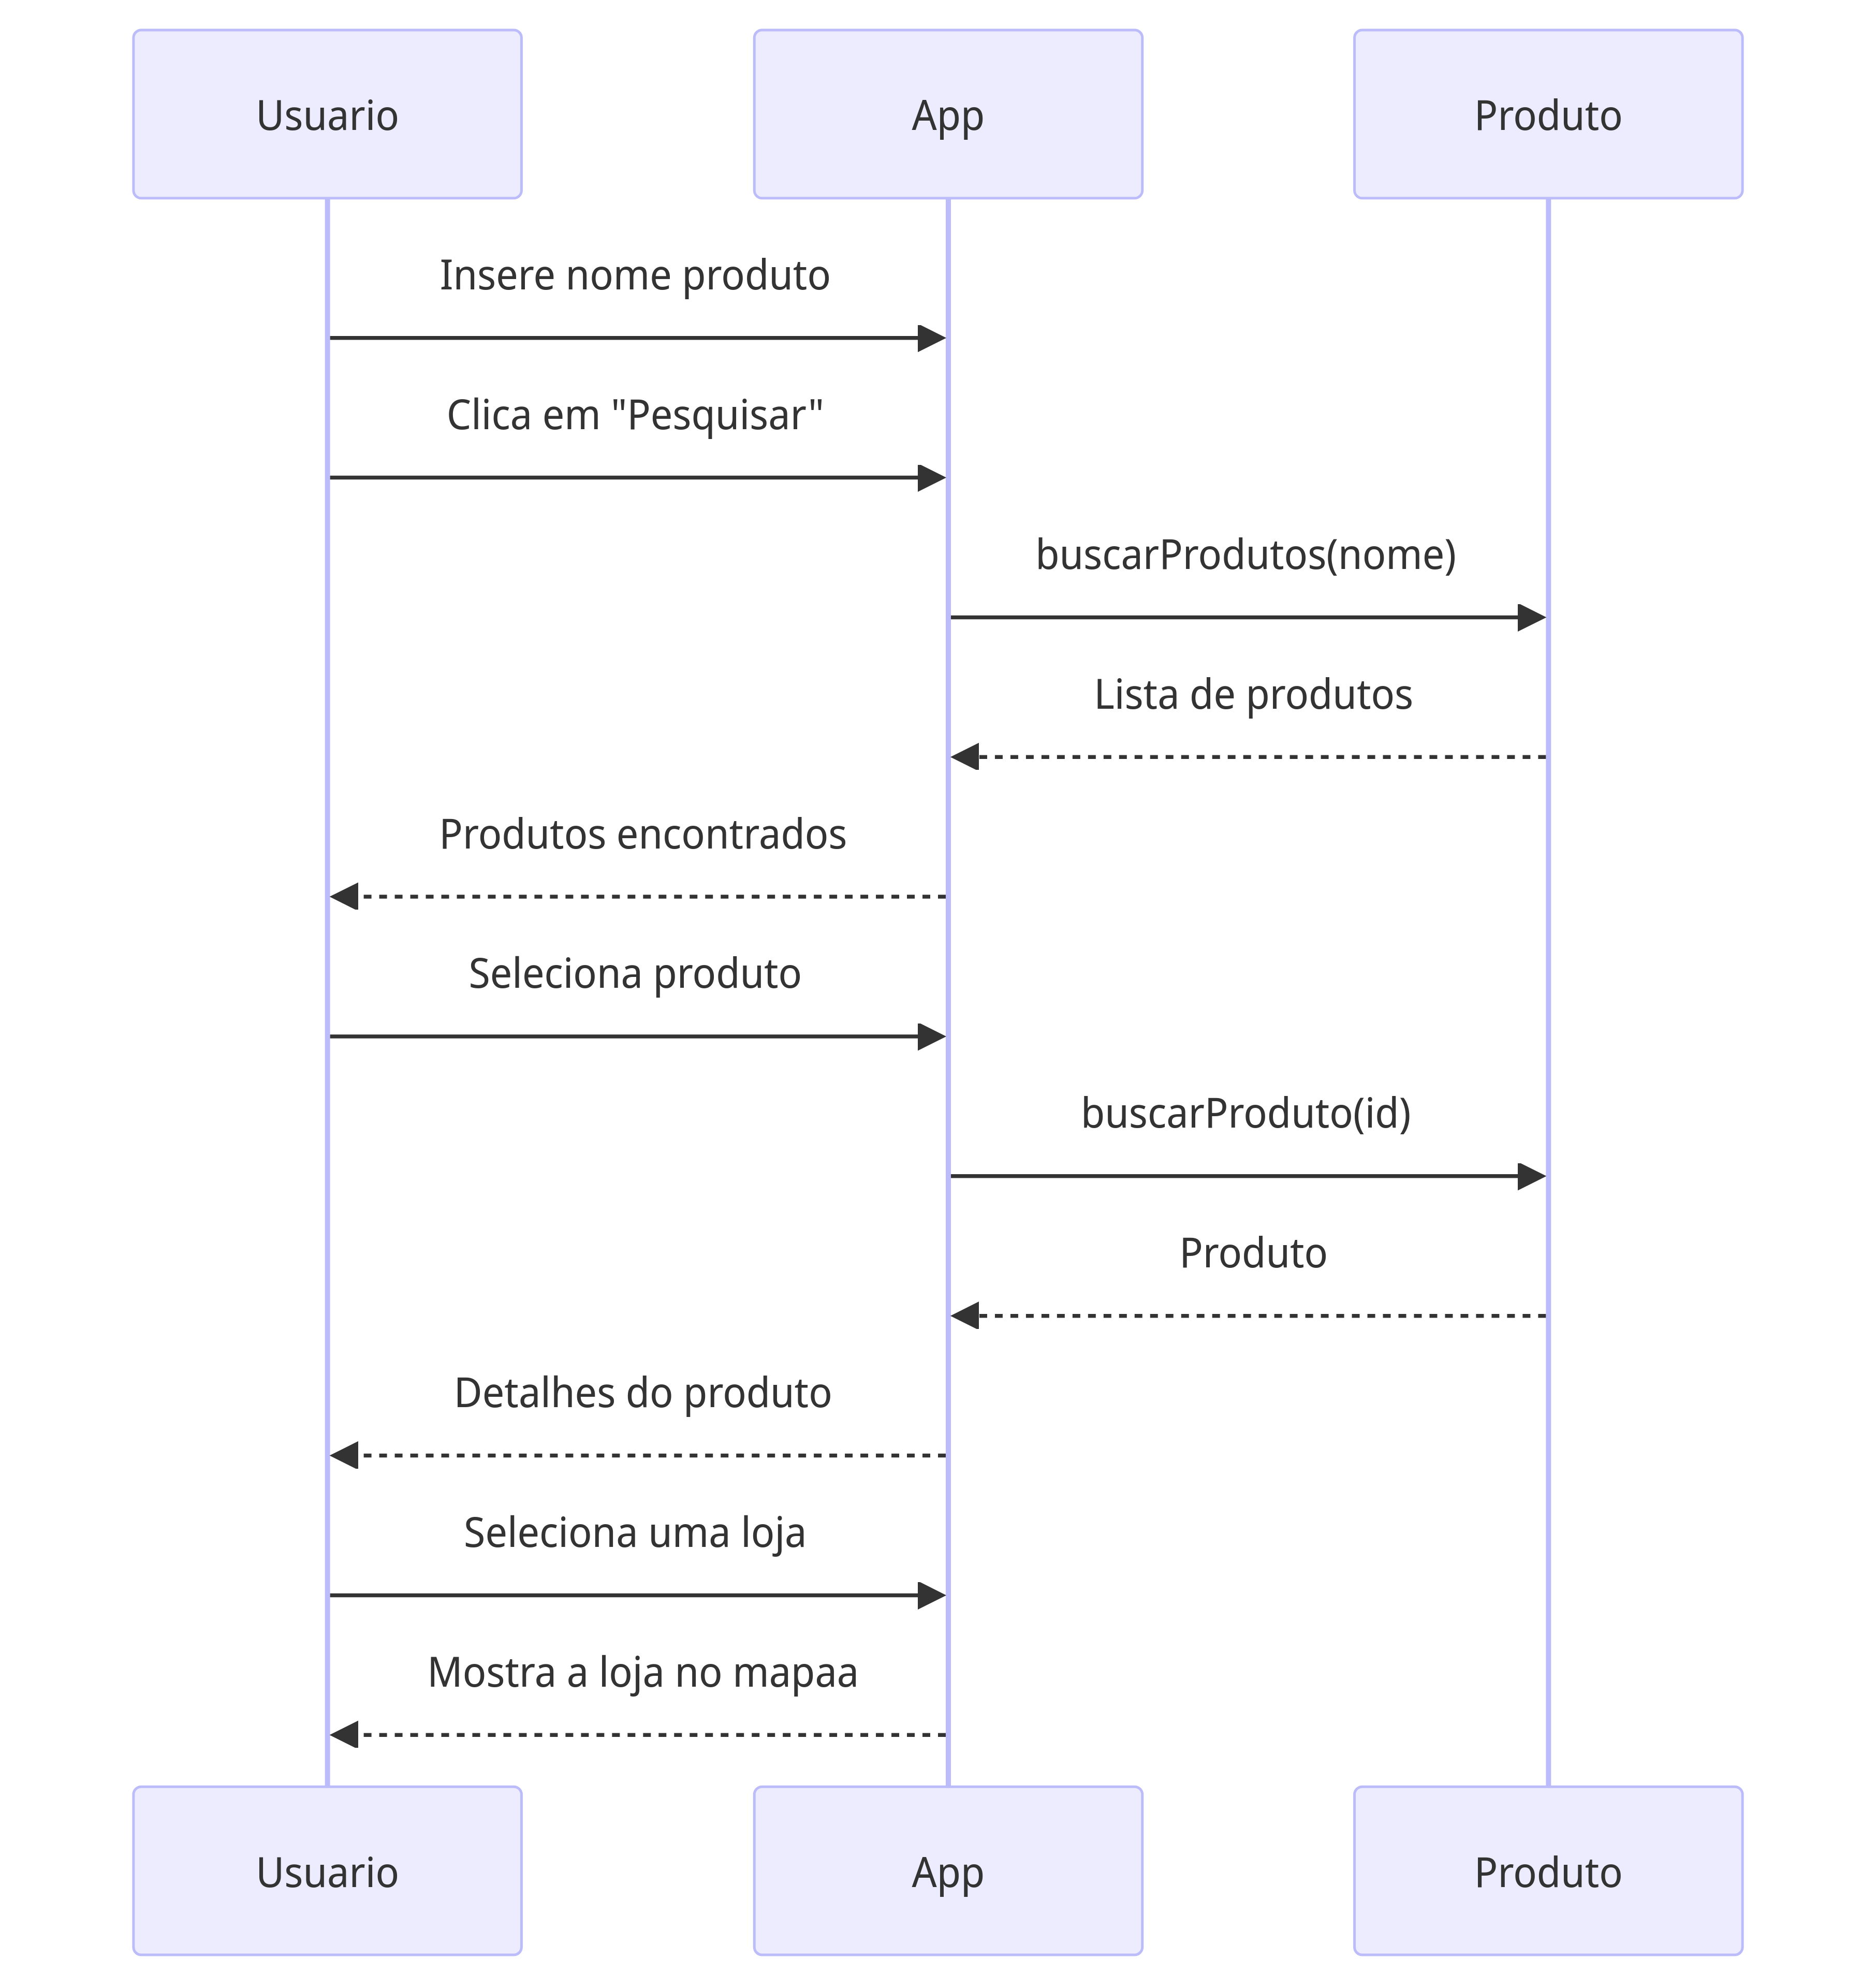
\includegraphics[width = 150mm]{fig/sequencia/sequencia1.png}
    \footnotesize \centering
    \par FONTE: O Autor (2024)
\end{figure}

\section{Avaliar sugestão}
\begin{figure}[H]
    \caption{\label{fig:label} DIAGRAMA DE SEQUÊNCIA AVALIAR SUGESTAO}
    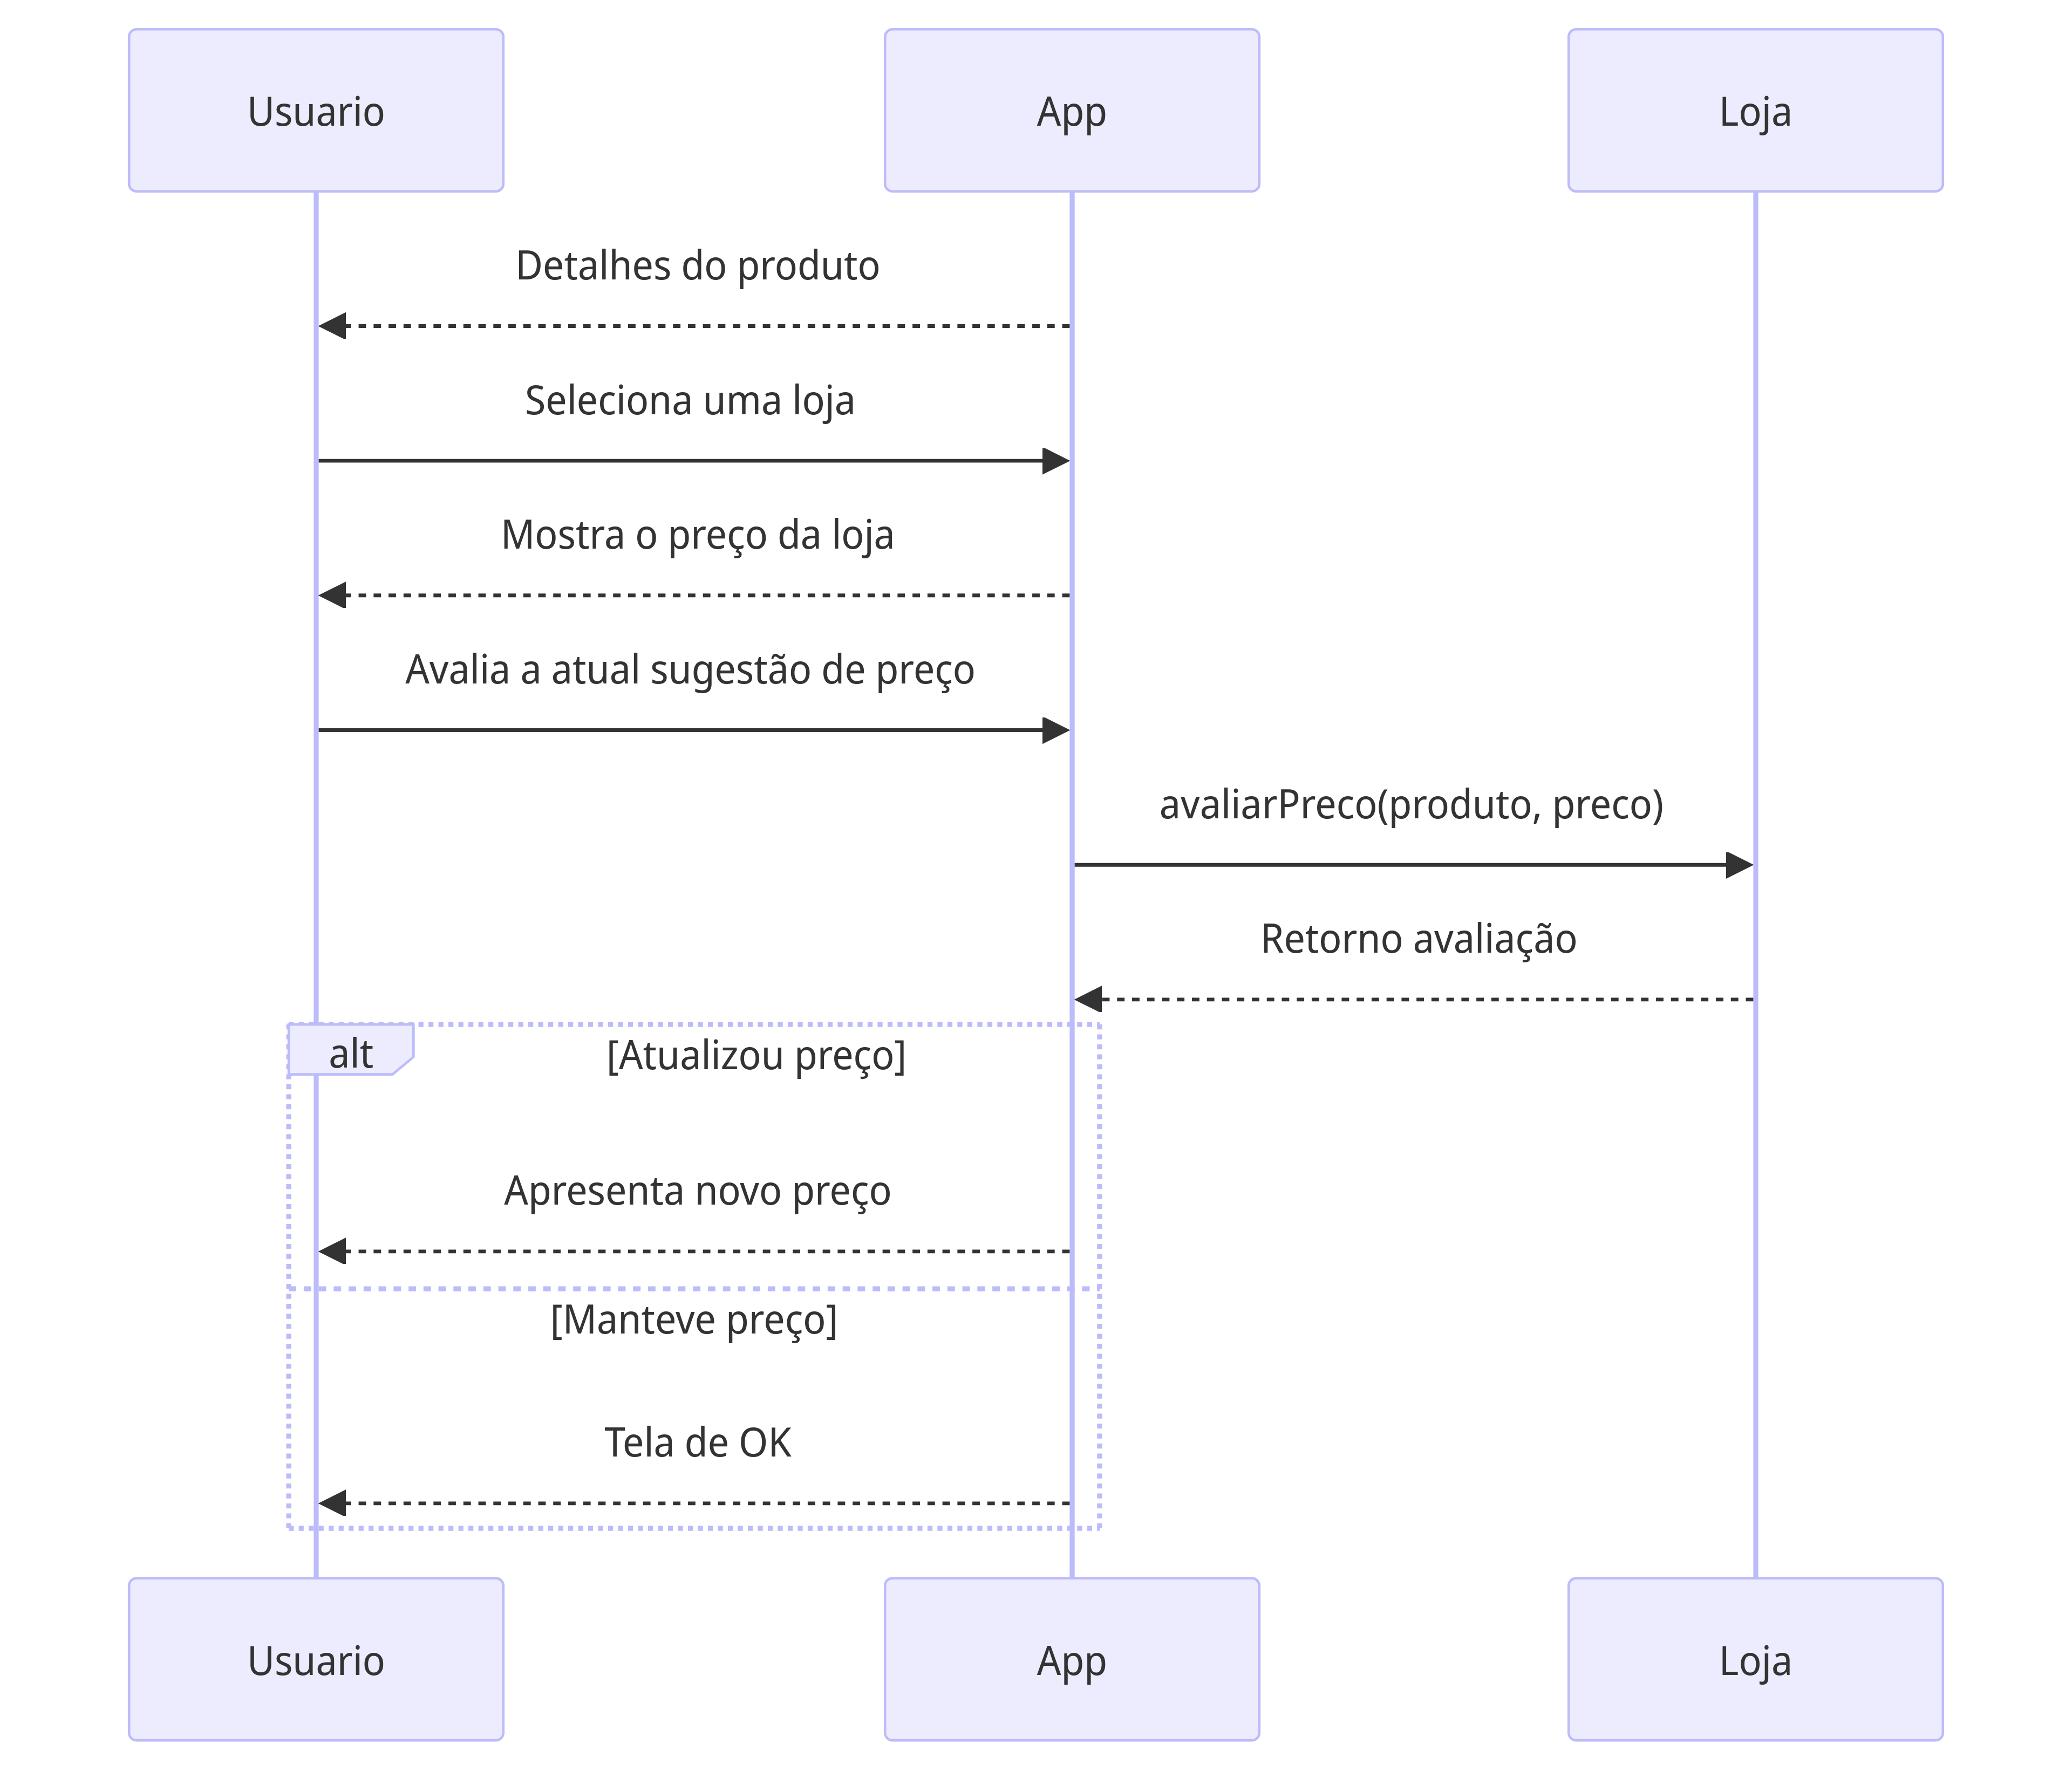
\includegraphics[width = 150mm]{fig/sequencia/sequencia2.png}
    \footnotesize \centering
    \par FONTE: O Autor (2024)
\end{figure}


\section{Sugerir edição}
\begin{figure}[H]
    \caption{\label{fig:label} DIAGRAMA DE SEQUÊNCIA SUGERIR EDIÇÃO}
    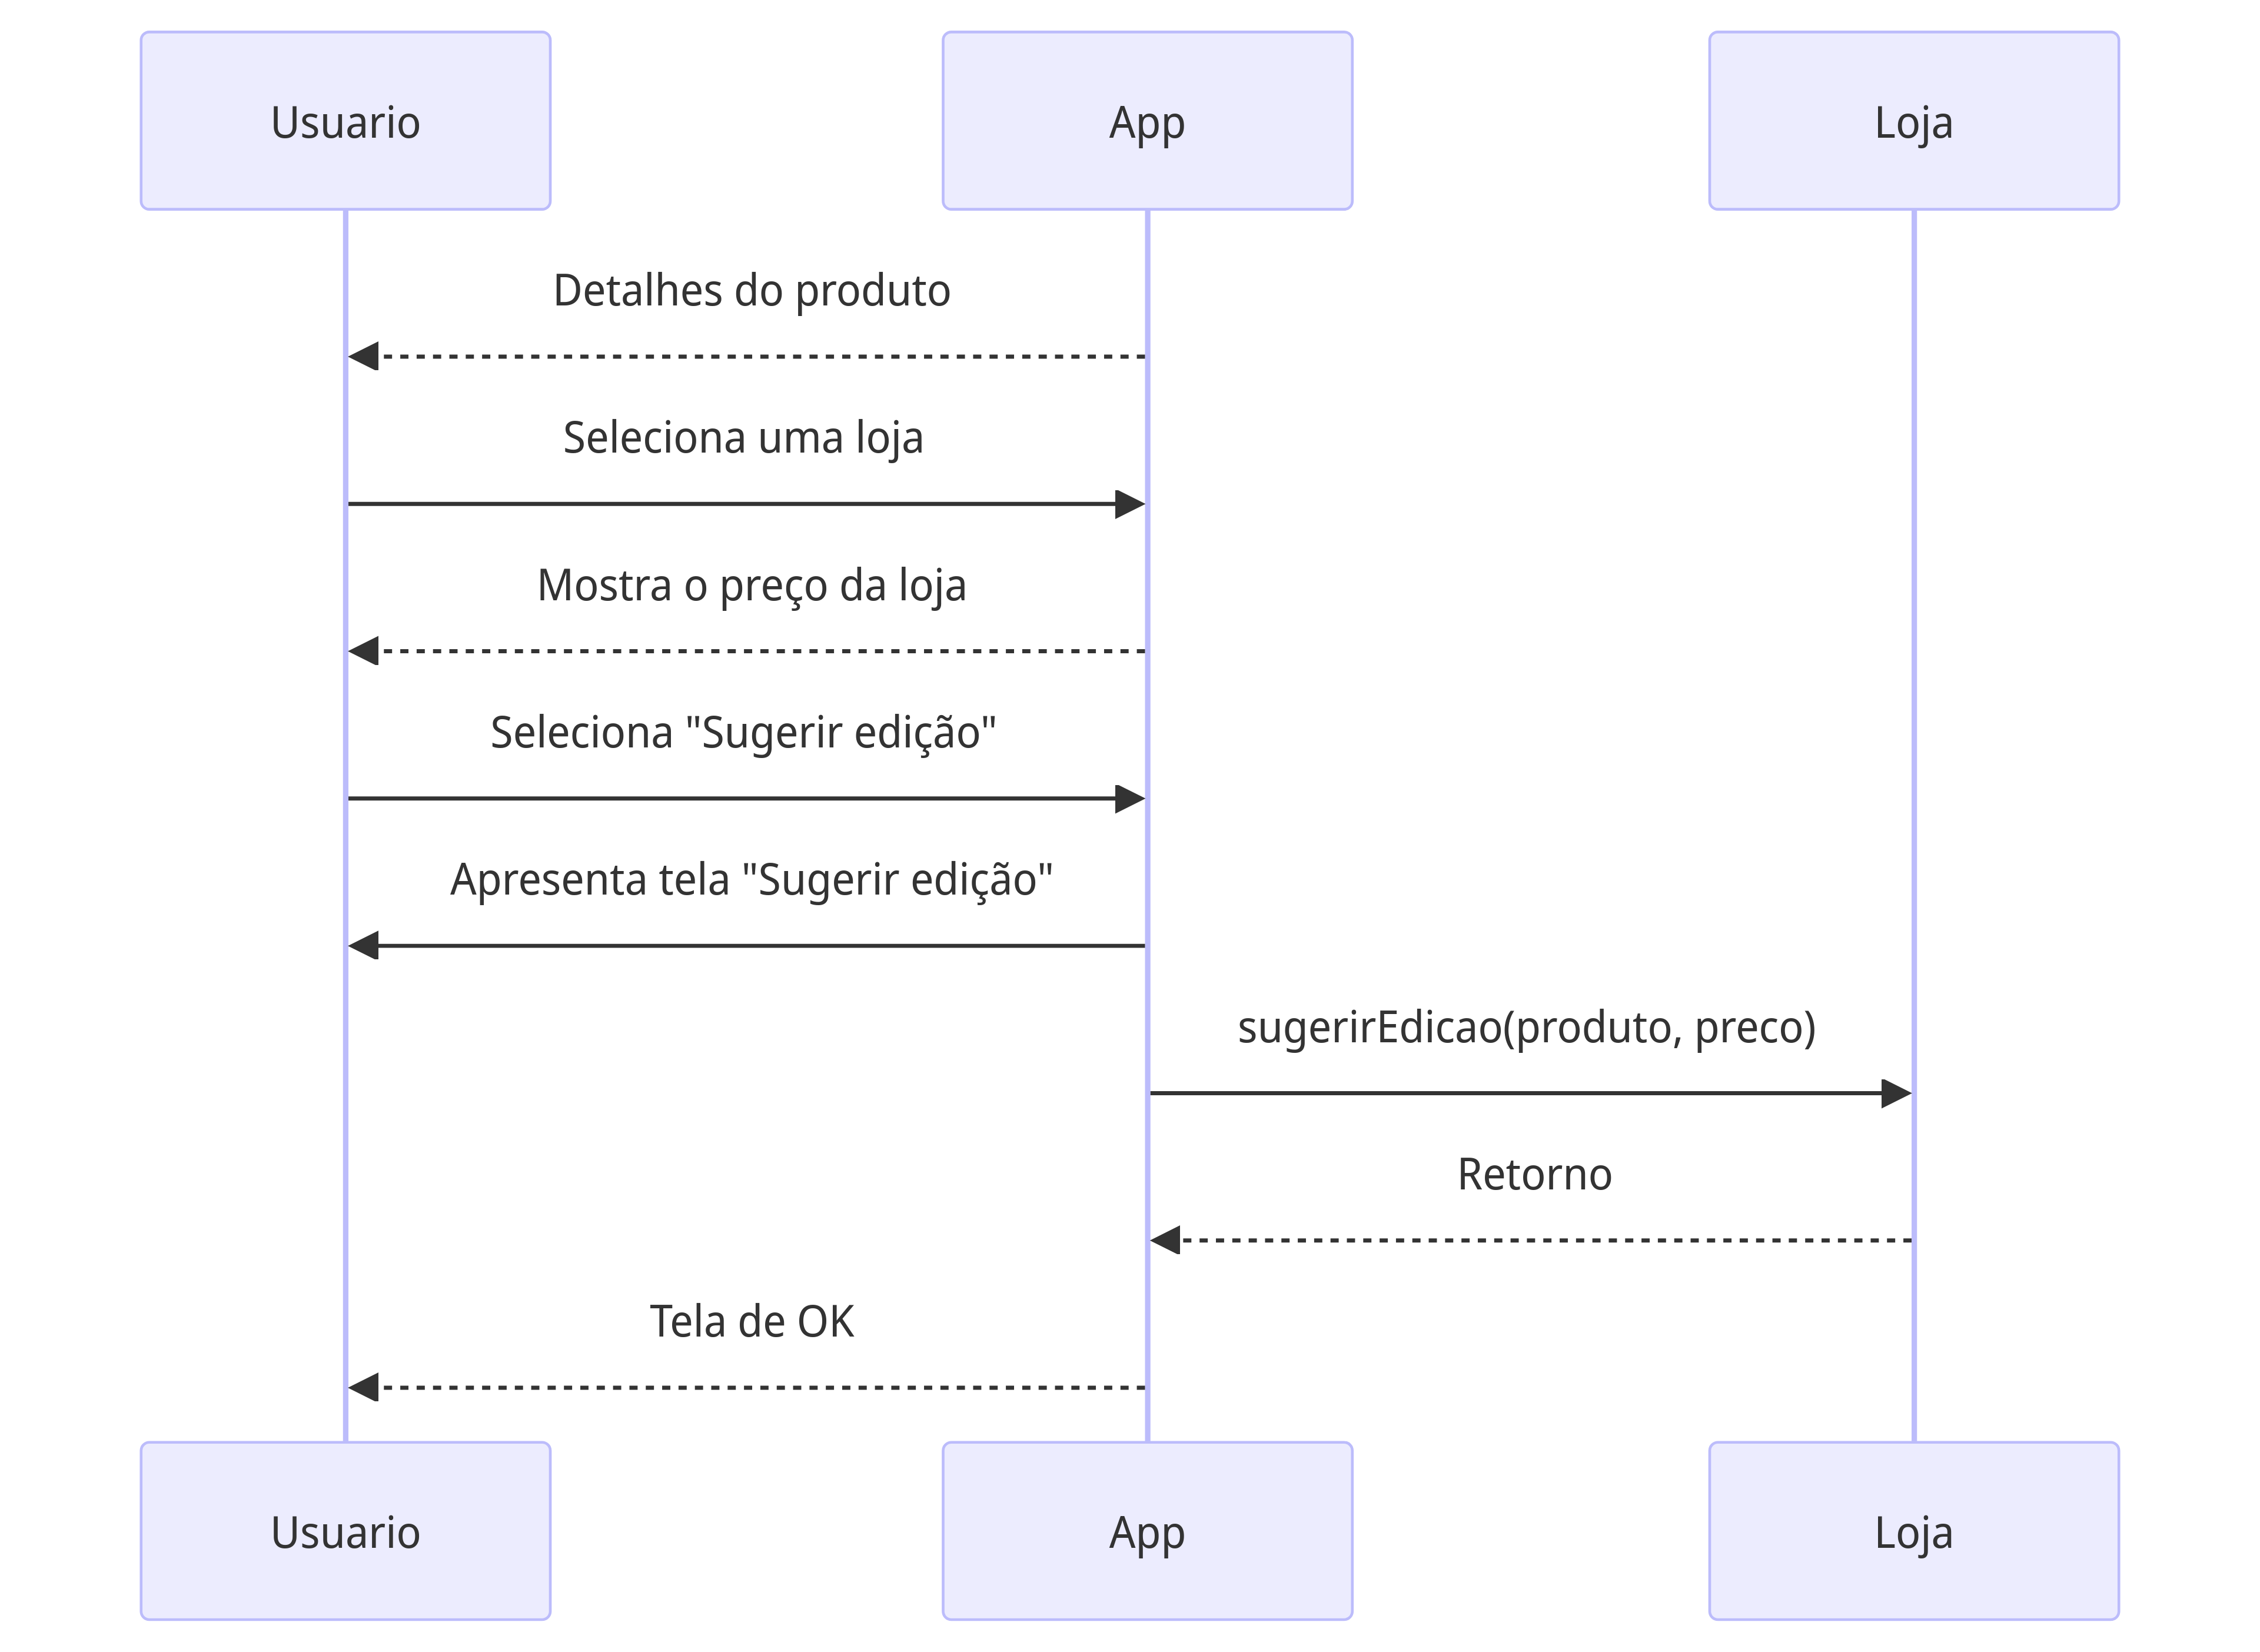
\includegraphics[width = 150mm]{fig/sequencia/sequencia3.png}
    \footnotesize \centering
    \par FONTE: O Autor (2024)
\end{figure}

\section{Cadastrar produto}
\begin{figure}[H]
    \caption{\label{fig:seqcadprod} DIAGRAMA DE SEQUÊNCIA CADASTRAR PRODUTO}
    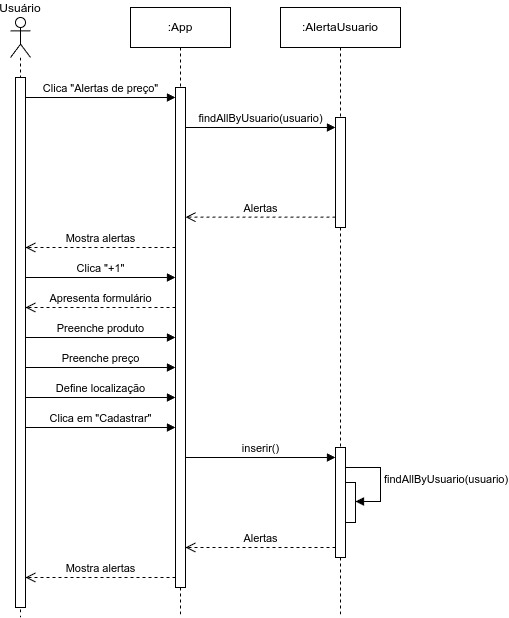
\includegraphics[width = 150mm]{fig/sequencia/sequencia4.png}
    \footnotesize \centering
    \par FONTE: O Autor (2024)
\end{figure}


%\section{Alterar senha}


%\section{Adicionar produto favorito}


%\section{Logar no sistema}


%\section{Criar conta}


%\section{Recuperar senha}